


\section{Non-normal Data}

\begin{frame}
  \begin{center}
    {\bf Part I -- Dealing with Non-normal Data}
  \end{center}
\end{frame}

\begin{frame}{Non Normality}{What is non-normality?}
  \begin{itemize}
    \item Until now we studied test statistics which assume that the {\bf estimator} calculated from the sample comes from a normal distribution (or close enough).\bigskip
    \item In some cases, this assumption {\bf does not hold}. In this condition,
      how can we perform the statistical analysis of the results?
  \end{itemize}
\end{frame}

\subsection{Motivation Example}

\begin{frame}[fragile]{Non Normal data make everything different}{Weight Loss Example}
A researcher is examining two different diets, {\bf Diet A} and {\bf Diet B},
and wants to compare the weight loss by people following one diet or the other.
They obtained the following data:

\begin{verbatim}
diet.a <- c(4,3,0,-3,-4,-5,-11,-14,-15,-300)
diet.b <- c(-8,-10,-12,-16,-18,-20,-21,-24,-26,-30)
\end{verbatim}
\bigskip

As you can see, Diet A has one big outlier that makes the data not normal. How much does this affect the statistical test?\bigskip

{\smaller
\begin{block}{Note!}
  Remember that in real research we need to ask ourselves: Why does this outlier exist? Is it an error in the experiment? An error in the data input? A new discovery? This is part of research!
\end{block}}

\end{frame}

\begin{frame}{Non Normal data make everything different}{The visualization of the data is very different with and without the outlier.}
  \begin{columns}
    \column{.5\textwidth}
    Data with Outlier\\
    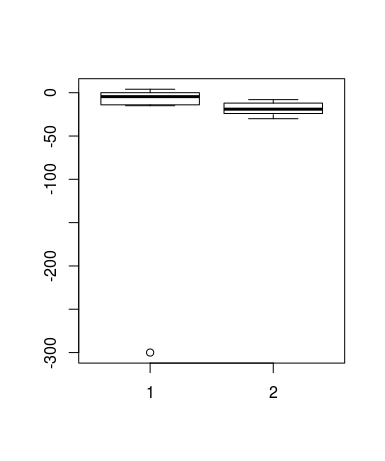
\includegraphics[width=.8\textwidth]{../img/diet_outlier1}
    \column{.5\textwidth}
    Data without Outlier\\
    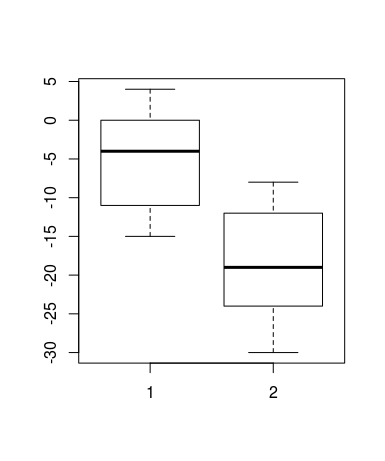
\includegraphics[width=.8\textwidth]{../img/diet_outlier2}
  \end{columns}\bigskip

  Checking a visualization, it seems like diet A has smaller losses than diet B
  overall. Except for that outlier. What happens with the T-test?
\end{frame}

\begin{frame}[fragile]{Non Normal data make everything different}
  {The outlier influences the result of the t-test}

The standard T-test does not indicate a difference between these samples,
and even suggests that the mean of the first sample is lower!\bigskip

{\smaller
\begin{verbatim}
diet.a <- c(4,3,0,-3,-4,-5,-11,-14,-15,-300)
diet.b <- c(-8,-10,-12,-16,-18,-20,-21,-24,-26,-30)
t.test(diet.a,diet.b)

##  Welch Two Sample t-test
## data:  diet.a and diet.b
## t = -0.53945, df = 9.1048, p-value = 0.6025
## alternative hypothesis: true difference in means is not equal to 0
## 95 percent confidence interval:
##  -82.9774  50.9774
## sample estimates:
## mean of x mean of y
##     -34.5     -18.5
\end{verbatim}}
\end{frame}


\begin{frame}{Non Normal data make everything different}{What can we do about it?}

  \begin{itemize}
    \item Should we find and remove outliers?
    \begin{itemize}
      \item If the outlier is an experimental error, it makes sense to remove it;
      \item Sometimes, the outlier is a important effect that needs to included in the analysis;
    \end{itemize}
    \bigskip

    \item It is also possible to use statistical methods that are not sensitive to the outlier.
  \end{itemize}

\end{frame}


\begin{frame}[fragile]{Non Normal data make everything different}{Non-parametric methods}

{\bf Non-parametric tests} use statistics that come from \structure{non-parametric distributions}.
\bigskip

In this case, a non-parametric test will indicate the difference between the {\bf location shift} of the two samples (i.e., the first sample has smaller observations than the second).

{\small
\begin{verbatim}
diet.a <- c(4,3,0,-3,-4,-5,-11,-14,-15,-300)
diet.b <- c(-8,-10,-12,-16,-18,-20,-21,-24,-26,-30)
wilcox.test(diet.a,diet.b)

##  Wilcoxon rank sum test
##
## data:  diet.a and diet.b
## W = 82, p-value = 0.01469
##
## alternative hypothesis: true location shift is not equal to 0
\end{verbatim}}
\end{frame}

\subsection{Concepts and Examples}

\begin{frame}{Examples of Non-Normal Data}
  There are many different ways that data can violate the assumption of normality:\bigskip

  \begin{itemize}
    \item \emph{Special Observations in the Data}:
      \begin{itemize}
        \item Outliers, data collection errors;
        \item Absolute limits in the data (measuring time);
      \end{itemize}

    \item \emph{Extreme Non-Normal Distributions:}
    \begin{itemize}
      \item Power Distribution, Cauchy Distribution, etc.
    \end{itemize}

    \item \emph{Ordinal Data:}
    \begin{itemize}
      \item Ordinal data is data that can be ordered and compared by some criteria, but you cannot apply traditional algebra on it (ex: subjective scores);\hfill $\leftarrow$\alert{Important!}
    \end{itemize}

    \item \emph{Completely Non-numerical data}:
    \begin{itemize}
      \item categorical data, class data, etc; (ex: colors)
    \end{itemize}
  \end{itemize}
\end{frame}


\begin{frame}{Non-Normal Data Example: Random Processes}

  Random processes in nature, such as plant growth or shell formation, are often seen to follow a normal distribution or bell curve.\bigskip

  On the other hand, {\bf random artificial processes not always follow a normal}.\bigskip

  \begin{itemize}
    \item In general, Pseudo Random Number Generators will use an {\bf Uniform Distribution}. Because of the CLT, aggregations of these results will tend to normal distributions.\medskip

    \item On the other hand, random social processes will often show {\bf Power Distributions} (salaries, social networks) or {\bf Binomial Distributions} (queues);\medskip

    \item It is important to study and understand the process being researched to know its characteristics;
  \end{itemize}
\end{frame}

\begin{frame}{Non Normal Data Example: Likert Data}
% TODO: Add a slide or section about how we should deal with
% LIKERT data.

\structure{Likert} data is the format often collected from surveys and interview questions.\medskip

\begin{center}
  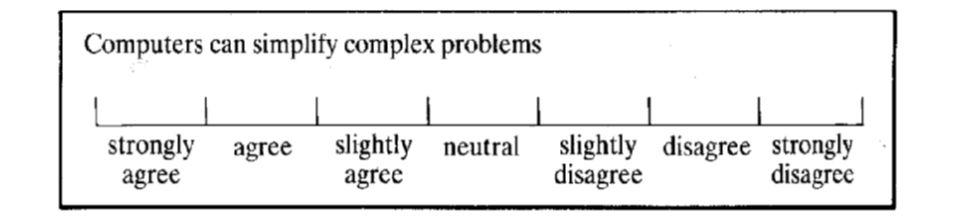
\includegraphics[width=0.8\textwidth]{../img/likert_scale}
\end{center}

Why can't we treat likert data directly as numerical? A few reasons:
\begin{itemize}
  \item Values outside of the 0-5 range have no meaning;
  \item Algebra on likert data has no meaning (Example: Neutral$+$Disagree$=$???)
  \item The difference between levels is not clear.
  \begin{itemize}
    \item Is "slightly agree" closer to "agree" or closer to "neutral"?
  \end{itemize}
\end{itemize}
\end{frame}

% \begin{ftstf}{Non Normality}{Example: Fully Symbolic Data}
% TODO: Expand on this example
%   Some data may not have a clear numerical correspond
% \end{ftstf}

\subsection{Strategies}
\begin{frame}{Strategies for working with Non-Normal data}
  When our data does not follow the normality assumption, there are many different strategies that we can apply, depending on the type of data, and the type of normality violation:\bigskip

  \begin{itemize}
    \item {\bf Do Nothing}
    \begin{itemize}
      \item We can just remove the outliers that break the normality assumption;
      \item We can trust that test will be robust for small deviations of normality;
    \end{itemize}
    \item {\bf Transform the Data}
      \begin{itemize}
        \item Transformation of the data can restore the normal property to data;
      \end{itemize}
    \item {\bf Non parametric Testing}
    \begin{itemize}
      \item Some statistical tests do not assume normal data (in exchange for smaller power);
    \end{itemize}
    \item {\bf Look for a new statistics textbook}
    \begin{itemize}
      \item There are entire books dedicated to the analysis of non-normal data.
    \end{itemize}
  \end{itemize}\bigskip

\end{frame}

% TODO: DO NOTHING SECTION
%    - remove outliers
%    - Trusting the CLT
%    - You need to understand WHY your data is not normal ()
% TODO: How to report on non-normal data
% TODO: FIXME: separate the lecture in *skewed* data and *ordinal* data.
% \begin{ftstf}{Non Normality}{Reporting on non-normal data} %% What you need to write on the paper
%   \begin{itemize}
%     \item Mean, Median, Ranks
%     \item Standard Deviation and IQR
%   \end{itemize}
% \end{ftstf}
%
% TODO: When is it ok to ignore small violations of normality?
% \section{Do nothing}
%
% \begin{ftstf}{Strategy 1 - Do nothing}{Ignoring the assumption of normality.}
%   \begin{itemize}
%     \item Very high number of samples is available (how high?);
%     \item The other conditions must still hold;
%   \end{itemize}
% \end{ftstf}
% TODO: R-code: some normal data with high n do not pass a normality test.
% findNonNormal <- function(n = 5000){
%     p <- 1
%     while(p > 0.05) {
%         y <- rnorm(n)
%         p <- shapiro.test(y)$p.value
%         }
%     y
%     }
%
% y <- findNonNormal()
% hist(y)
% qqnorm(y)


%\section{Data Transformation}

\begin{frame}[fragile]{Data Transformation}{Using Log Transformation to transform from Lognormal to Normal distribution}
  \begin{columns}
    \column{0.6\textwidth}
    \begin{center}
      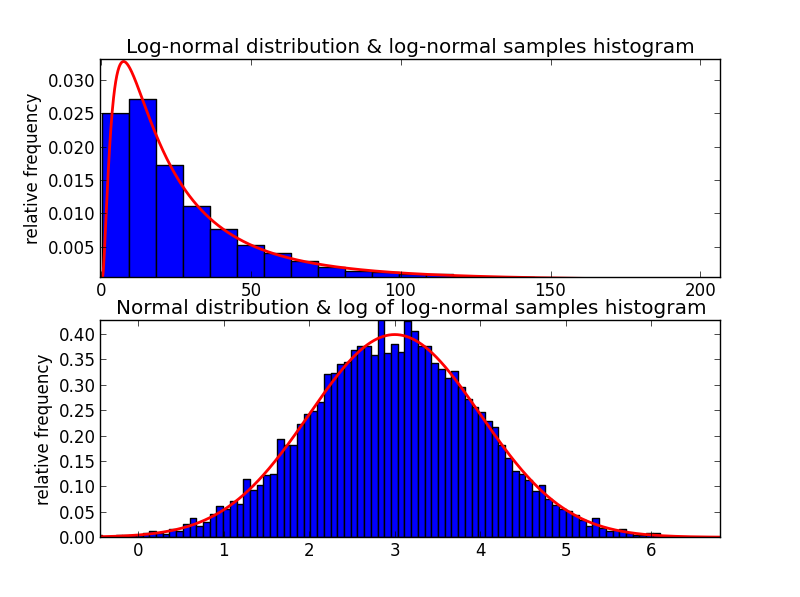
\includegraphics[width=1\textwidth]{../img/lognormal_transformation}
    \end{center}
    \column{0.4\textwidth}
{\smaller
\begin{verbatim}
# R Example of log transform:

# example lognormal data
z <- exp(rnorm(200, -2, 0.4))

# Log transformation
y <- log(z)

# Normal estimators
# from lognormal data:
mu.hat <- mean(y)
sigma.hat <- sd(y)
\end{verbatim}}
  \end{columns}
\end{frame}


\begin{frame}{Data Transformation}{Skew Transformation}
  A strong skew in the sampling distribution can be a larger problem for the standard statistical tests. It is possible to remove these through data transformations:\bigskip

  \begin{itemize}
    \item For left skewed data:
    \begin{itemize}
      \item square root, cube root, log
    \end{itemize}
    \item For right skewed data:
    \begin{itemize}
      \item square root (constant $-x$), cube root (constant $-x$)
    \end{itemize}
  \end{itemize}\bigskip

  {\bf Attention:} The logarithm of 0 and negative data is not defined. If your data includes 0 or negatives, you may need to add a constant before the transformation.
\end{frame}
% TODO: Example of transformation to remove skew



\begin{frame}{Data Transformation}{Be careful when transforming data}
  \begin{itemize}
    \item Pay attention when describing the analysis on a paper or report:
    \begin{itemize}
      \item When you talk about the analysis, you need to explain the transformation used;

      \item When you discuss the results, you must consider the transformed data, as well as the original data;

      \item In particular, the {\bf Meaningful difference} must be discussed on the original data;
    \end{itemize}\bigskip

    \item Beware that the hypotheses may not be equivalent!
    \begin{itemize}
      \item Example: The lognormal mean includes the variance. But the transformed lognormal mean does not. In this case, the null hypothesis is only equivalent when the variance of the transformed distribution is equal!
    \end{itemize}
  \end{itemize}
\end{frame}
%% TODO: Example of the mistakes above -- what wrong conclusions you can reach if you don't do this.

\subsection{Bootstrapping}

\begin{frame}{Bootstrapping}{Using the CLT to make the data more normal}

  The Bootstrapping procedure is used to obtain an approximation of the "sample mean distribution" from the sample data.\bigskip

  By the Central Limit Theorem, the sample mean distribution of a random variable will usually follow a normal distribution; even when the underlying distribution of observation values is not normal;\bigskip

  So how can we use this to transform non-normal data?
\end{frame}

\begin{frame}{The Bootstrapping Procedure}
  \begin{itemize}
    \item Take an initial sample with $m$ observations;
    \item Create $n$ {\bf bootstrap samples} by selecting $m_b < m$ from the initial sample $n$ times;
    \item Calculate the mean of each bootstrap sample.

    \begin{center}
      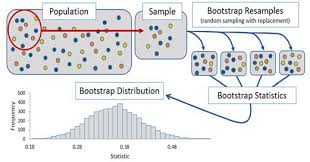
\includegraphics[width=.7\textwidth]{../img/bootstrap_lowres}
      % TODO: Redo picture or find source.
    \end{center}
  \end{itemize}
\end{frame}



\begin{frame}[fragile]{Generating Bootstrapped Data}
  {R Package "boot" for bootstrapping, confidence intervals, and tests.}
  \begin{columns}[T]
    \column{0.7\textwidth}
    {\smaller
\begin{verbatim}
% Non-normal data:
> city
    1    2    3    4    5    6    7    8    9   10
u 138   93   61  179   48   37   29   23   30    2
x 143  104   69  260   75   63   50   48  111   50

% We are interested in the ratio of u and x
> ratio <- function(d, w) sum(d$x * w) / sum (d$u * w)

% Using library boot to create bootstrapped data:
> library(boot)
> bootstrap <- boot(city, ratio, R = 999, stype = "w")
> bootstrap.city <- bootstrap[[2]]
\end{verbatim}
    }
    \column{0.3\textwidth}
    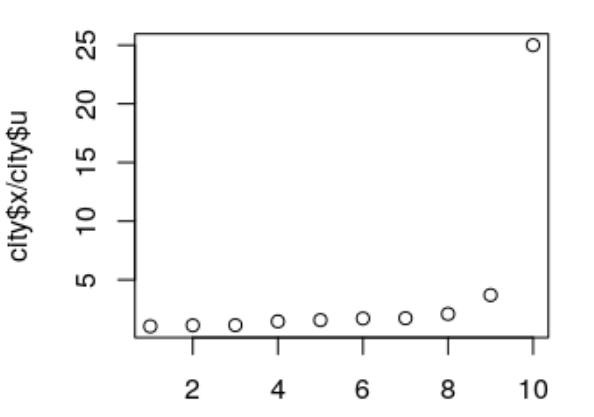
\includegraphics[width=.9\textwidth]{../img/bootstrap_original}
    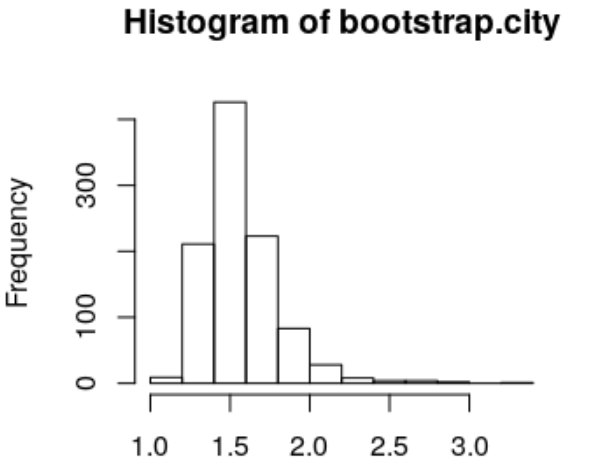
\includegraphics[width=.9\textwidth]{../img/bootstrap_histogram}
  \end{columns}
\end{frame}

\subsection{Non-Parametric Tests}

\begin{frame}{Non Parametric Tests}{}
  Non-parametric Tests involve statistics that do not assume normality from the population distribution.\bigskip

  Weak assumptions about the population, however, causes the non-parametric tests to be less strong than parametric ones. Also, usually non-parametric statistics usually do not calculate the distance between the parameter estimate and the hypothesis values.
  \bigskip

  \begin{itemize}
    \item Wilcoxon Signed Rank Test (1 sample)
    \item Wilcoxon Ranked Sum Test / Mann-whitney Test (2 samples)
    \item Kruskall-Wallis Test (multiple samples)
  \end{itemize}
\end{frame}

% \begin{frame}{Non Parametric Tests}{Basic Idea}
%   % TODO: Generally explain the basic idea of non-parametric tests
% \end{frame}

\subsection{Non-Parametric test, 1 or 2 samples}

% \begin{frame}{Non Parametric Tests}{One or two Samples}
%   \begin{itemize}
%     \item unpaired test: Mann-Whitney U-test;
%     \item paired test: Wilcoxon signed-ranks test;
%   \end{itemize}
% \end{frame}

\begin{frame}{Mann-Whitney U-test}{Unpaired test for two samples}
  \begin{center}
    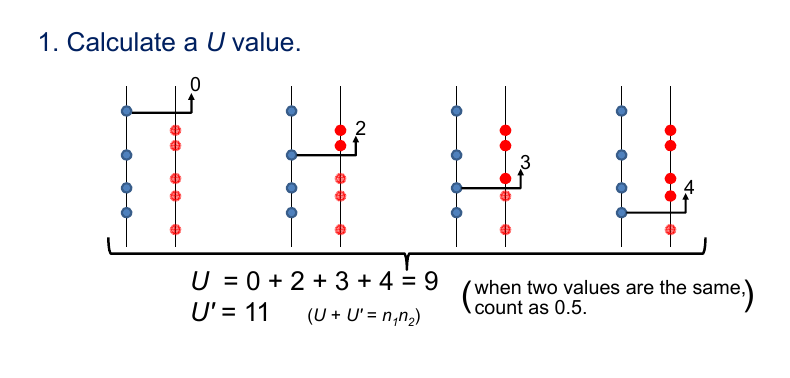
\includegraphics[width=1\textwidth]{../img/MannWhitneyU}
  \end{center}
\end{frame}

\begin{frame}{Mann-Whitney U-test}{}
  \begin{center}
    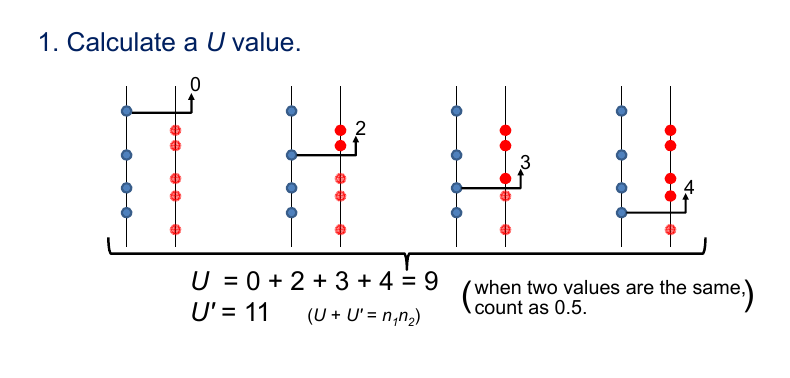
\includegraphics[width=.5\textwidth]{../img/MannWhitneyU}
  \end{center}

  \begin{itemize}
    \item Choose the smaller value of U or U'
    \item Null Hypothesis: {\bf Both samples come from the same distribution}
    \item Under the null hypothesis, for big enough $n_1$ and $n_2$, U follows
    roughly a normal distribution with mean $\frac{n_1n_2}{2}$ and variance $\frac{n_1n_2(n_1+n_2+1)}{12}$
    \item Calculate the test statistic z, and find the p-value from the $\alpha$-percentile in the z distribution.
  \end{itemize}
\end{frame}

\begin{frame}{Wilcoxon Signed Rank Test}{}
  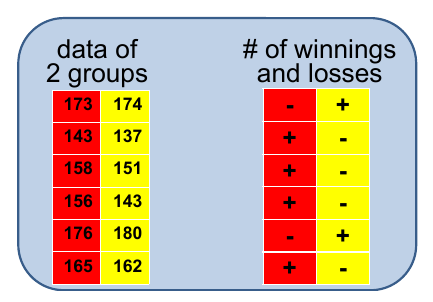
\includegraphics[width=.4\textwidth]{../img/SignTest}

  \begin{itemize}
    \item The Wilcoxon test takes the relative difference between pairs (positive or negative)
    \item Null hypothesis: {\bf Positive and Negative signs are equally likely}
    \item The overall number of signs is compared against a binomial distribution under the Null hypothesis.
  \end{itemize}
\end{frame}


\begin{frame}[fragile]{Wilcoxon Signed Rank Test}{R code example}

{\smaller
\begin{verbatim}
## Hollander & Wolfe (1973), 29f.
## Hamilton depression scale factor measurements in 9 patients with mixed anxiety
## and depression, taken at the first (x) and second (y) visit after initiation
## of a therapy (administration of a tranquilizer).

# Data:
% x <- c(1.83,  0.50,  1.62,  2.48, 1.68, 1.88, 1.55, 3.06, 1.30)
% y <- c(0.878, 0.647, 0.598, 2.05, 1.06, 1.29, 1.06, 3.14, 1.29)

# Running the test:
% wilcox.test(x, y, paired = TRUE, alternative = "greater")

Wilcoxon signed rank test
data:  x and y
V = 40, p-value = 0.01953
alternative hypothesis: true location shift is greater than 0
\end{verbatim}}
\end{frame}

\subsection{Recommended Reading}
\begin{frame}{Recommended Reading}{}

  {\smaller
  \begin{itemize}
    \item Kristin L Sainani, "Dealing with Non-Normal Data."\\ \url{https://onlinelibrary.wiley.com/doi/full/10.1016/j.pmrj.2012.10.013}
    \item Feng et al., "Log transformation and its implication for data analysis."\\ \url{https://www.ncbi.nlm.nih.gov/pmc/articles/PMC4120293/}
    \item Bommae Kim, "Should I always Transform My Variables to Make them Normal?"\\ \url{https://data.library.virginia.edu/normality-assumption/}
%    \item Hideyuki Takagi, "Tutorial on Statistical Tests"\\ \url{http://www.design.kyushu-u.ac.jp/~takagi/TAKAGI/downloadablefile.html\#StatisticalTests}
  \end{itemize}}

\end{frame}
